\chapter{Einleitung}
\label{ch:intro}
Die Helvetia ist ein schweizerisches Versicherungsunternehmen, welches schon seit 1858 operiert. \cite{Helv}
Über die Jahre hat Helvetia ein Hostsystem verwendet, um die Daten der Nutzer zu speichern und auswerten zu können.
In dieser Zeit ist der Host stetig gewachsen mit der Helvetia.
Dies hatte zur Folge, dass die Berechtigungsstruktur der Helvetia im Hostbereich immer komplexer wurde.
Zudem wurde dieser nur selten überprüft und auf dem neuesten Stand gehalten.
Dies hat das Problem verschlimmert.
Durch die steigende Komplexität wird es schwieriger, mit der Berechtigungsstruktur umzugehen.
Dabei ist dies problematisch, da die Mitarbeiter über diese Berechtigungsstruktur rezertifiziert werden.
Daher muss die Berechtigungsstruktur modernisiert werden, damit die Verwendung dieser keine Probleme darstellt.

\section{Motivation für die Arbeit}
\label{sec:intro:motivation}
Viele Unternehmen verfügen über sensible Informationen, beispielsweise Versicherungen oder Krankenhäuser.
Sensible Informationen können dabei Telefonnummern oder auch Namen und Adressen sein.
Diese Informationen werden auf gesicherten Servern gelagert, auf welche nur bestimmte Personen Zugriffsberechtigungen haben.
Diese Personen verfügen über Profile, die ihnen diese Berechtigungen zur Verfügung stellen.
Jedoch kann es passieren, dass solche Profile gestohlen oder Personen gegeben werden, welche diese nicht haben dürfen.
Berechtigungsstrukturen sollen genau diese Szenarien verhindern.
Wird aber eine Berechtigungsstruktur lange genutzt und werden nicht alle Richtlinien und Normen eingehalten, so wird diese im Laufe der Zeit unsicherer und unübersichtlicher.
Hierdurch steigt das Risiko, dass die sensitiven Informationen in nicht autorisierte Hände gelangen.
Dadurch können sogenannte "`Super Accounts"' entstehen.
"`Super Accounts"' verfügen über zu viele bis zu allen Berechtigungen im System.
Sollte diese Person durch einen Angriff diesen "`Super Account"' verlieren, wäre die gesamte Struktur kompromittiert.
Dasselbe ist der Fall, wenn ein Mitarbeiter mit einem solchen Account dem Unternehmen schaden will.

\begin{figure}[h!]
 \centering
 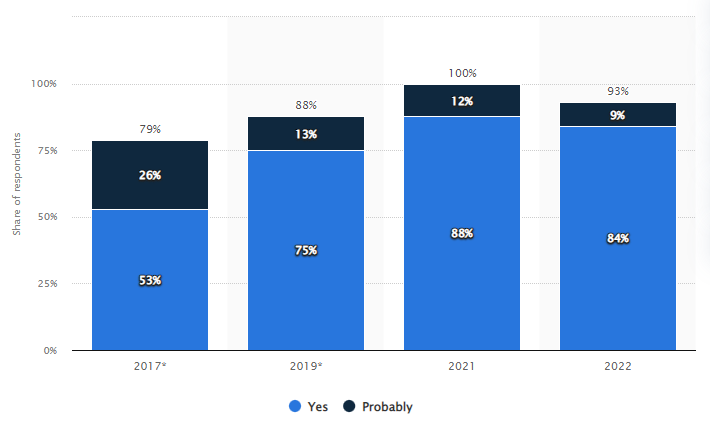
\includegraphics[width=1\textwidth]{gfx/Picture/Cyber_Crime.PNG}
 \caption{Eine Umfrage von deutschen Unternehmen, die von Daten Diebstahl, Spionage oder Sabotage betroffen waren. \cite{Stat22}}
 \label{fig:Crime}
\end{figure}

Wie man in der Grafik (\ref{fig:Crime}) erkennen kann, waren 88\% der befragten Unternehmen in Deutschland von Datendiebstahl, Spionage oder Sabotage in 2021 betroffen.
Im Jahr 2022 lag der Anteil bei 84\%.
Wobei man berücksichtigen muss, dass diese Befragung zwischen Januar und März stattgefunden hat und dies daher nur das erste Quartal von 2022 abdeckt.
Aufgrund dessen, dass solche Angriffe wahrscheinlich sind, sollte es keine "`Super Accounts"' geben, da diese ansonsten in solchen Angriffen als Schwachstelle ausgenutzt werden können.
Genauso müssen die Strukturen übersichtlich sein, damit es bei einer Überprüfung keine Probleme bei der Analyse gibt, welcher Nutzer welche Berechtigungen verfügt.
Wenn dies nicht der Fall ist, kann es passieren, dass die jeweiligen Nutzer zu viele Berechtigungen haben und so weitere Schwachstellen für Spionage oder Sabotage entstehen.
Um dies zu erreichen, gibt es verschiedene Methoden und Konzepte, die die Berechtigungsstrukturen sicher und übersichtlich gestalten.

%
% Section: Ziele
%
\section{Problem Spezifikation}
\label{sec:intro:UWD}
Für die Untersuchung der Probleme im Hostbereich wurden verschiedene Stakeholder interviewed und befragt.
Die gesammelten Ergebnisse bilden das folgende Ursache-Wirkungs-Diagramm in der Grafik (\ref{fig:Fisch})
\begin{figure}[h!]
 \centering
 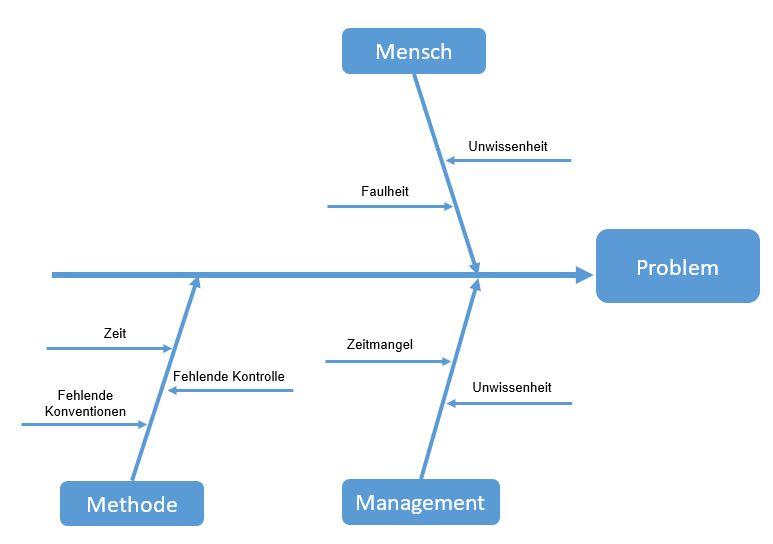
\includegraphics[width=1\textwidth]{gfx/Picture/Fisch.PNG}
 \caption{Ursache-Wirkungs-Diagramm (Fischgrätenmodell)}
 \label{fig:Fisch}
\end{figure}
Im Ursache-Wirkungs-Diagramm wurden dabei die folgenden drei Punkte als Hauptursache für das Problem der bestehenden Berechtigungsstruktur erkannt:
\begin{itemize}
	\item Mensch
	\item Management
	\item Methode
\end{itemize}
Hier bezeichnet Mensch diejenigen Mitarbeiter, welche die Berechtigungsstruktur verwalten und hegen.
Dort wurden die Punkte Faulheit und Unwissenheit genannt.
Es ist nicht unüblich, dass diese gewisse Formalien ignorieren, um einfacher das Problem zu beheben.
Auf der anderen Seite ist auch die Unwissenheit ein Problem, da die gesamte Struktur so gewachsen ist.
Dadurch ist es für jemanden unmöglich, diese komplett nachzuvollziehen.
\newline
Das Management hat nicht die Zeit, sich genau mit dem Problem zu beschäftigen.
Dies hat zur Folge, dass das Management wie die Mitarbeiter unwissend ist.
\newline
Bei der Methode stellt die Zeit, fehlende Kontrolle und fehlende Konventionen als Problem dar.
Mit der Zeit ist gemeint, dass die aktuelle Problemstellung schon so lange der Fall ist, dass dies ein Problem ist.
An vielen Stellen fehlt die Kontrolle bei der bestehenden Berechtigungsstruktur.
Dies ist zum Beispiel der Fall, wenn ein Account wieder aktiviert wird oder bei der Überprüfung von Profilen.
Denn wenn es diese gäbe, dürfte es keine rekursiven Beziehungen geben.
Es fehlt auch eine allgemeine Konvention, wie die Profile in den verschiedenen Fachbereichen funktionieren.
Dies sorgt dafür, dass es die Mitarbeiter schwerer haben alle Verbindungen zu verstehen und macht die gesamte Struktur komplexer.
\newline
Dies sind die bestehenden Ursachen, warum das aktuelle Problem mit der Berechtigungsstruktur im Host besteht.
Um das Problem beheben zu können, müssen einige dieser Unterprobleme behoben werden.
Da sowohl das Management noch der Mensch geändert werden kann, muss dementsprechend die Methode angepasst werden.
Dabei sind die Faktoren fehlende Kontrolle und fehlende Konvention, welche geändert werden können.
\newpage

\section{Ziel der Arbeit}
\label{sec:intro:goal}
Diese wissenschaftliche Ausarbeitung ist eine Vergleichsarbeit, bei der verschiedene Konzepte verglichen werden.
Dabei wird auf die folgende Fragestellung in dieser Arbeit eingegangen: \textit{inwieweit man bestehende Berechtigungsstrukturen im Hostbereich verändern und optimieren kann}.
Dazu gibt es drei Unterfragen, welche verwendet werden, um die Problemstellung systematisch zu beantworten.

\begin{itemize}
  \item \textit{Welche Konzepte und Standards werden derzeit für Berechtigungsstrukturen verwendet, um diese sicher und übersichtlich zu gestalten?}
  \item \textit{Wie unterscheiden sich die verschiedenen Konzepte?}
  \item \textit{Womit kann man die verschiedenen Konzepte vergleichen?}
\end{itemize}

Die erste Unterfrage wird durch eine Recherche mit verschiedenen Arbeiten im Bereich der Berechtigungsstruktur beantwortet.
Dabei werden auch die Best-Practise von verschiedenen Unternehmen betrachtet und analysiert.
Außerdem werden die Berechtigungsstrukturen von Datenbanken beleuchtet.
Dies soll einen Überblick zum Stand der Technik geben, um eine geeignete Lösung zu finden.
\newline
Anschließend wurden mehrere Befragungen durchgeführt, um die bestehenden Konzepte nach den Wünschen der Befragten anzupassen.
Diese Befragten sind die betroffenen Stakeholder.
Darauf basierend werden die bestehenden Methoden bewertet und verglichen.
Der Vergleich findet mithilfe von Nutzwertanalysen statt.
Dies beantwortet die zweite Unterfrage mithilfe des erstellten Vergleiches.
\newline
Um die dritte Frage zu beantworten, werden Analysetools verwendet, welche als eine Hilfestellung zur Konzeptauswahl dienen.
Mit diesen werden die verschiedenen Konzepte mit Punkten bewertet, um das bessere Konzept zu ermitteln.
Zum Schluss wird eine Alternative zum bestehenden System vorgestellt.
In der Grafik \ref{fig:vorgehen} ist der Aufbau der Arbeit schematisch dargestellt.
\newpage
\begin{figure}[h!]
\hspace*{-3cm}
 \centering
 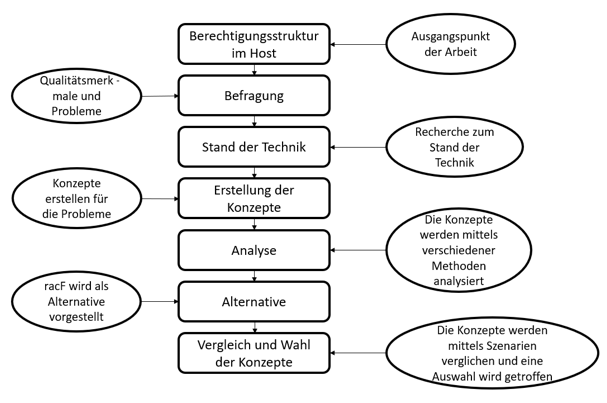
\includegraphics[width=1.5\textwidth]{gfx/Picture/Vorgehen.PNG}
 \caption{Aufbau der Arbeit}
 \label{fig:vorgehen}
\end{figure}